\documentclass[tikz,border=6pt]{standalone}
\usepackage{amsmath,amssymb}
\usetikzlibrary{arrows.meta}
\begin{document}
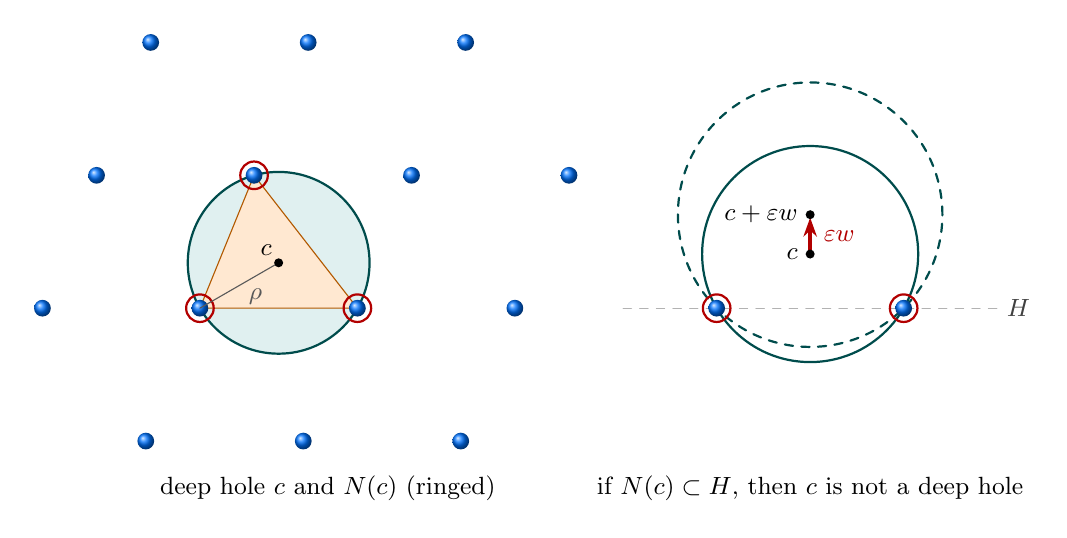
\begin{tikzpicture}[scale=1.25,line cap=round,>={Stealth[length=2.4mm,width=1.7mm]}]
  % left: a lattice, a deep hole c and the circle of radius rho about it
  \begin{scope}
  \clip (-1.75,-1.55) rectangle (4.0,2.85);
  \fill[teal!12] (0.8000,0.4611) circle (0.9234);
  \draw[teal!60!black,thick] (0.8000,0.4611) circle (0.9234);
  \fill[orange!18] (0,0)--(1.6,0.0)--(0.55,1.35)--cycle;
  \draw[orange!70!black,thin] (0,0)--(1.6,0.0)--(0.55,1.35)--cycle;
  \shade[ball color=blue!55!cyan] (-1.600,0.000) circle (0.085);
  \shade[ball color=blue!55!cyan] (-1.050,1.350) circle (0.085);
  \shade[ball color=blue!55!cyan] (-0.500,2.700) circle (0.085);
  \shade[ball color=blue!55!cyan] (-0.550,-1.350) circle (0.085);
  \shade[ball color=blue!55!cyan] (0.000,0.000) circle (0.085);
  \shade[ball color=blue!55!cyan] (0.550,1.350) circle (0.085);
  \shade[ball color=blue!55!cyan] (1.100,2.700) circle (0.085);
  \shade[ball color=blue!55!cyan] (1.050,-1.350) circle (0.085);
  \shade[ball color=blue!55!cyan] (1.600,0.000) circle (0.085);
  \shade[ball color=blue!55!cyan] (2.150,1.350) circle (0.085);
  \shade[ball color=blue!55!cyan] (2.700,2.700) circle (0.085);
  \shade[ball color=blue!55!cyan] (2.650,-1.350) circle (0.085);
  \shade[ball color=blue!55!cyan] (3.200,0.000) circle (0.085);
  \shade[ball color=blue!55!cyan] (3.750,1.350) circle (0.085);
  \draw[red!70!black,thick] (0.000,0.000) circle (0.14);
  \draw[red!70!black,thick] (1.600,0.000) circle (0.14);
  \draw[red!70!black,thick] (0.550,1.350) circle (0.14);
  \draw[gray!70!black] (0.8000,0.4611)--(0,0) node[pos=0.45,below right=-1.5pt,font=\small] {$\rho$};
  \fill[black] (0.8000,0.4611) circle (1.3pt) node[above left=-1pt,font=\small] {$c$};
  \end{scope}
  \node[font=\small,anchor=north] at (1.3,-1.6) {deep hole $c$ and $N(c)$ (ringed)};
  % right: if N(c) lay in a hyperplane, moving c away from it would increase the distance
  \draw[gray!60,dashed] (4.300000000000001,0)--(8.1,0) node[right,font=\small,gray!50!black] {$H$};
  \draw[teal!60!black,thick] (6.2,0.55) circle (1.0977);
  \draw[teal!60!black,thick,dashed] (6.2,0.95) circle (1.3435);
  \draw[->,red!70!black,very thick] (6.2,0.55)--(6.2,0.9199999999999999) node[pos=0.5,right=1pt,font=\small] {$\varepsilon w$};
  \shade[ball color=blue!55!cyan] (5.250,0.000) circle (0.085);
  \draw[red!70!black,thick] (5.250,0.000) circle (0.14);
  \shade[ball color=blue!55!cyan] (7.150,0.000) circle (0.085);
  \draw[red!70!black,thick] (7.150,0.000) circle (0.14);
  \fill[black] (6.2,0.55) circle (1.3pt) node[left=1pt,font=\small] {$c$};
  \fill[black] (6.2,0.95) circle (1.3pt) node[left=1pt,font=\small] {$c+\varepsilon w$};
  \node[font=\small,anchor=north] at (6.2,-1.6) {if $N(c)\subset H$, then $c$ is not a deep hole};
\end{tikzpicture}
\end{document}
